\PassOptionsToPackage{unicode=true}{hyperref} % options for packages loaded elsewhere
\PassOptionsToPackage{hyphens}{url}
%
\documentclass[
  ignorenonframetext,
]{beamer}
\usepackage{pgfpages}
\setbeamertemplate{caption}[numbered]
\setbeamertemplate{caption label separator}{: }
\setbeamercolor{caption name}{fg=normal text.fg}
\beamertemplatenavigationsymbolsempty
% Prevent slide breaks in the middle of a paragraph:
\widowpenalties 1 10000
\raggedbottom
\setbeamertemplate{part page}{
  \centering
  \begin{beamercolorbox}[sep=16pt,center]{part title}
    \usebeamerfont{part title}\insertpart\par
  \end{beamercolorbox}
}
\setbeamertemplate{section page}{
  \centering
  \begin{beamercolorbox}[sep=12pt,center]{part title}
    \usebeamerfont{section title}\insertsection\par
  \end{beamercolorbox}
}
\setbeamertemplate{subsection page}{
  \centering
  \begin{beamercolorbox}[sep=8pt,center]{part title}
    \usebeamerfont{subsection title}\insertsubsection\par
  \end{beamercolorbox}
}
\AtBeginPart{
  \frame{\partpage}
}
\AtBeginSection{
  \ifbibliography
  \else
    \frame{\sectionpage}
  \fi
}
\AtBeginSubsection{
  \frame{\subsectionpage}
}
\usepackage{lmodern}
\usepackage{amssymb,amsmath}
\usepackage{ifxetex,ifluatex}
\ifnum 0\ifxetex 1\fi\ifluatex 1\fi=0 % if pdftex
  \usepackage[T1]{fontenc}
  \usepackage[utf8]{inputenc}
  \usepackage{textcomp} % provides euro and other symbols
\else % if luatex or xelatex
  \usepackage{unicode-math}
  \defaultfontfeatures{Scale=MatchLowercase}
  \defaultfontfeatures[\rmfamily]{Ligatures=TeX,Scale=1}
\fi
% use upquote if available, for straight quotes in verbatim environments
\IfFileExists{upquote.sty}{\usepackage{upquote}}{}
\IfFileExists{microtype.sty}{% use microtype if available
  \usepackage[]{microtype}
  \UseMicrotypeSet[protrusion]{basicmath} % disable protrusion for tt fonts
}{}
\makeatletter
\@ifundefined{KOMAClassName}{% if non-KOMA class
  \IfFileExists{parskip.sty}{%
    \usepackage{parskip}
  }{% else
    \setlength{\parindent}{0pt}
    \setlength{\parskip}{6pt plus 2pt minus 1pt}}
}{% if KOMA class
  \KOMAoptions{parskip=half}}
\makeatother
\usepackage{xcolor}
\IfFileExists{xurl.sty}{\usepackage{xurl}}{} % add URL line breaks if available
\IfFileExists{bookmark.sty}{\usepackage{bookmark}}{\usepackage{hyperref}}
\hypersetup{
  pdftitle={How to write an R package and publish it on GitHub},
  pdfauthor={Aya Mitani},
  pdfborder={0 0 0},
  breaklinks=true}
\urlstyle{same}  % don't use monospace font for urls
\newif\ifbibliography
\setlength{\emergencystretch}{3em}  % prevent overfull lines
\providecommand{\tightlist}{%
  \setlength{\itemsep}{0pt}\setlength{\parskip}{0pt}}
\setcounter{secnumdepth}{-2}

% set default figure placement to htbp
\makeatletter
\def\fps@figure{htbp}
\makeatother

\usetheme[progressbar=frametitle]{metropolis}
\usepackage{graphicx}
\usepackage{rotating}
\usepackage{amsmath}
\usepackage{float}
\usefonttheme[onlymath]{serif}
\AtBeginPart{}
\AtBeginSection{}
\AtBeginSubsection{}
\AtBeginSubsubsection{}
\usepackage{multicol}
\newcommand{\btwocol}{\begin{multicols}{2}}
\newcommand{\etwocol}{\end{multicols}}

\title{How to write an R package and publish it on GitHub}
\author{Aya Mitani}
\date{2021/01/07}

\begin{document}
\frame{\titlepage}

\begin{frame}{What is R package?}
\protect\hypertarget{what-is-r-package}{}

\begin{itemize}
\tightlist
\item
  Collection of code, data, documentation developed by R community
\item
  Addresses particular problem with specialised statistical technique,
  graphical device, etc.
\item
  Core set of packages come with base R
\item
  \(>\) 15,000 Additional packages available from CRAN, Bioconductor,
  Omegahat, GitHub, etc.
\item
  Popular R packages

  \begin{itemize}
  \tightlist
  \item
    dplyr
  \item
    ggplot2
  \end{itemize}
\end{itemize}

\begin{figure}
  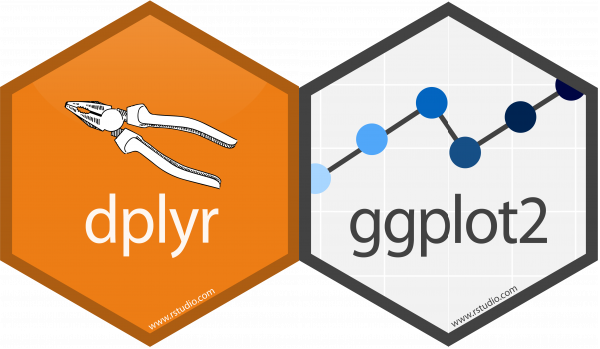
\includegraphics[scale=0.2]{slides_files/figure-beamer/dplyrggplot2.png}
\end{figure}

\end{frame}

\begin{frame}{What is GitHub?}
\protect\hypertarget{what-is-github}{}

\begin{itemize}
\tightlist
\item
  Website that hosts software development and version control using Git
\item
  Free basic services
\end{itemize}

\end{frame}

\hypertarget{why-write-r-package}{%
\subsection{\#\#\# Why write R package?}\label{why-write-r-package}}

\begin{itemize}
\tightlist
\item
  Increasingly, (bio)statistical journals ask for R package development
  of novel method
\end{itemize}

\begin{frame}{Why publish package on GitHub?}
\protect\hypertarget{why-publish-package-on-github}{}

\begin{itemize}
\tightlist
\item
  Reproducibility
\item
  Accessibility
\item
  Collaboration
\item
  Back-up method
\end{itemize}

\end{frame}

\begin{frame}{What do you need to write R package?}
\protect\hypertarget{what-do-you-need-to-write-r-package}{}

\begin{itemize}
\tightlist
\item
  R
\item
  R Studio very useful
\item
  devtools package
\item
  GitHub account
\end{itemize}

\end{frame}

\begin{frame}{Let's begin!}
\protect\hypertarget{lets-begin}{}

\end{frame}

\end{document}
